\section{Syscall per la gestione dei processi in UNIX}
\subsection{Descrizione generale di UNIX}
UNIX è un sistema operativo multiprogrammato basato su processi.
I processi hanno spazio per i dati privato quindi possono comunicare tramite scambio di messaggi, mentre la porzione di codice può essere condivisa tra istanze diverse dello stesso programma, in questo modo si ottimizza la memoria.

UNIX ha uno scheduling a divisione di tempo ed i processi evolvono attraverso questa sequenza di stati:
\begin{figure}[H]
    \centering
    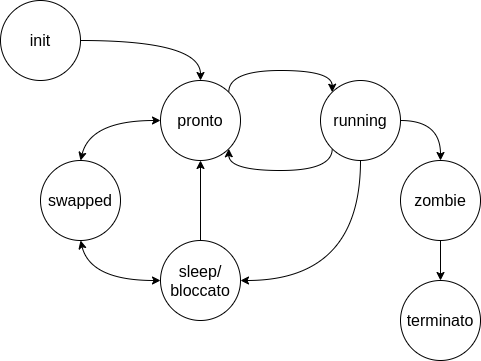
\includegraphics[width=300px]{images/1L_Syscall_UNIX_per_i_processi/stati_processo_unix.png}
\end{figure}
Si è in stato swapped quando il processo è stato stoppato e la sua memoria spostata su disco.
Si è in zombie quando un processo termina, se ne preservano alcune informazioni affinché il processo padre possa leggerle, una volta effettuata la lettura si va in terminato e si libera completamente la memoria dedicata alla gestione di quel processo.

Il PCB di un processo UNIX è diviso in due strutture:
\begin{itemize}
    \item process structure: usato per mantenere in memoria le informazioni indispensabili del processo.
    E' sempre in memoria principale.
    
    \item user structure: contiene informazioni utili solo quando il processo è residente in memoria.
    Subisce swap-out come la memoria del processo.
\end{itemize}

\subsection{Syscall}
\subsubsection{fork}
Serve a creare un processo figlio e può essere eseguita da qualsiasi processo a qualsiasi livello di privilegio.
Quando il processo figlio viene creato lo si crea come copia del padre, ha quindi uno spazio di memoria diverso ma che è la copia di quello del padre.
Il codice invece è condiviso in quanto eseguono lo stesso programma.
I figli a loro volta possono generare altri figli in modo da creare una gerarchia di processi.
\begin{verbatim}
    pid_t fork(void)
\end{verbatim}
Restituisce un intero che può essere:
\begin{itemize}
    \item 0: nel processo figlio
    \item un intero: nel processo padre, ed indica il pid del processo figlio.
    Oppure un numero negativo se la fork ha fallito.
\end{itemize}

NB: si noti che il tipo pid\_t non è standard del C, è un tipo definito (tipo opaco) a parte dalla libreria standard in modo da liberare il programmatore dal sapere quale sia l'effettivo tipo di ritorno.
Questo permette di scrivere codice più portabile su diversi dispositivi in quanto usiamo l' astrazione fornita da chi ha scritto la libreria.

All' interno di un processo possiamo scoprire il proprio pid usando:
\begin{verbatim}
    pid_t getpid()
\end{verbatim}
oppure il pid del processo padre con:
\begin{verbatim}
    pid_t getppid()
\end{verbatim}

\subsubsection{exit}
Un processo può terminare in maniera:
\begin{itemize}
    \item involontaria: se esegue azioni illegali come accedere ad indirizzi non mappati o eseguire istruzioni protette, oppure attraverso interruzioni causate da segnali esterni come SIGINT e SIGKILL
    
    \item volontariamente: usando la syscall exit
\end{itemize}
\begin{verbatim}
    exit(int status_code)
\end{verbatim}
exit non ha valore di ritorno in quanto causa la terminazione del processo, prende un parametro che è il codice di ritorno del processo, utilizzabile per comunicare l' esito del programma al processo padre.

\subsubsection{wait}
Quando un processo termina il suo processo padre può utilizzare la syscall wait per ottenerne lo status\_code.
\begin{verbatim}
    pid_t wait(int *status)
\end{verbatim}
Il suo valore di ritorno è il pid del processo terminato e passandogli un puntatore ad intero vi scriverà all' interno lo status\_code del processo terminato.

Può avere 3 comportamenti:
\begin{itemize}
    \item ritorna un valore negativo se non ci sono figli

    \item sospende il processo che la invoca finché uno dei figli non entra in stato zombie

    \item se quando è stata invocata c' era già un processo in stato zombie ne restituisce il PID
\end{itemize}

Lo status\_code è un valore usato per codificare il tipo di terminazione e la motivazione: se il byte meno significativo è 0 allora la terminazione è stata volontaria ed in questo caso il byte più significativo contiene lo stato di terminazione.

Le implementazioni potrebbero cambiare tra le varie versioni, quindi possiamo affidarci a delle macro di sistema:
\begin{verbatim}
    WIFEXITED(status)
        // ritorna vero se il processo è
        // terminato volontariamente
    
    WEXITSTATUS(status)
        // ritorna lo stato di terminazione
\end{verbatim}

\subsubsection{exec**}
Per sostituire il codice ed i dati del processo si può usare una delle syscall della famiglia exec**.
In particolare la versione execl:
\begin{verbatim}
    int execl(char* path, char* arg0, _, char* argN, NULL)
        // path è il percorso dell'eseguibile da lanciare
        // arg0 è il nome del comando, per convenzione
        // ag1:argN è l'elenco dei parametri
        // 0 è il terminatore della lista di parametri
\end{verbatim}
La chiamata ad exec è senza ritorno se ha successo, in quanto modifica il codice del processo ed il suo stato, se invece fallisce continua l' esecuzione del programma corrente quindi il valore di ritorno può essere usato per fare error handling.

